\chapter{Technology Review}

\begin{figure}[h!]
	\caption{AF Date Control Logo}
	\label{image:AF-Date-Control}
	\centering
	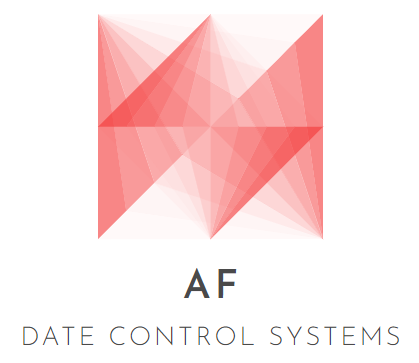
\includegraphics[width=0.55\textwidth]{images/AF-Date-Control.png}
\end{figure}

\subsection{The How and Why}
\begin{figure}[h!]
	\caption{Quotation From: https://www.brainyquote.com/}
	\label{image:quote1}
	\centering
	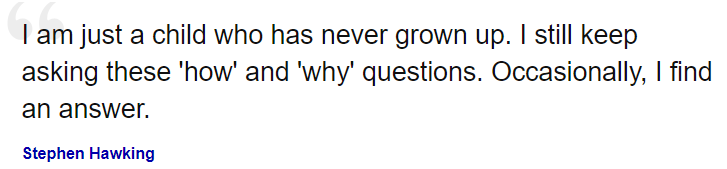
\includegraphics[width=0.8\textwidth]{images/quote1.PNG}
\end{figure}

With new ideas comes an influx of questions, the main two being the how and the why. How this idea came about ? this idea came about after five years of working part-time in retail. Looking at the day to day operations of the shop and what can i try and improve with what i have learned in college for four years, in this case i highlighted one area of the shop that i could integrate into my final year project and that is to develop an application to ease the burden of Date Checking for my fellow staff members. The human eye cannot spot everything, this would save time and money for the staff and shop as a whole respectively. The good thing also about this idea is the fact that it can be very flexible and can be made into various different types of applications with minor tweaks. This is a major characteristic that companies and retailers demand, versatility. It can help in many different ways.
\newline

So why this particular application and why would it be purposeful in the industry of retail. This interesting piece \cite{gustavsson2011global} provides incentive information about the global food wastage problem, this application will address this issue not just locally but globally. This piece proves it is an issue worldwide and with this application i hope that it can be a massive help in reducing this worrying statistic and flatten the curve of this problem as food wastage is still on the rise. This will help staff in finding the products before they go out of date and take action. Be it reducing that particular item or using that product for something in the shop, for example identifying a packet of sausages or rashers and putting giving them to the deli staff to cook and sell in the hot deli. This is a norm in the shop i currently work in part time and i feel this is making a difference however more can be done like always. Of course you are not going to be able to give every product close to it's sell by date to the deli or reduce it. This isn't going to solve the issue entirely but help it as much as it can. 

\subsection{Beneficial and Sufficient}
Before pursuing a Date Control Application for Retail, i wanted to know would it be beneficial to staff members and superiors in the workplace. I conducted a minor survey enclosed within my workplace to get some feedback for this potential idea. Which i will show the results in the Surveys section below. I personally believe this application idea will be very beneficial and sufficient for retailers across the country and even beyond and the good thing about this application is that it is not intense or in anyway complicated it is basic and easy to use for the staff member or user. It is not made to look exquisite it is made to solve or help an global issue in food wastage and to save shops time and money.
\newline

Outside of retail can this be beneficial and sufficient to other industries or organisations ? I very much think so. I feel it can be beneficial to the likes of charities and food banks. Items that may not be eligible for returns for credits can be donated to food banks or charities or even compost companies. \cite{riches1986food} Here is an interesting read on food banks and the welfare crisis in which it looks at the benefits of food banks for society. This is one of the many reasons why food wastage is a global issue that i hope this basic but sufficient application can address and aid in diluting these issues. 
\newline

\begin{figure}[h!]
	\caption{CBE Provides Shop Databases and Tills}
	\label{image:cbe}
	\centering
	
\includegraphics[width=0.35\textwidth]{images/cbe.jpg}
\end{figure}

The purpose of this application other than helping the retailers directly is offering this idea or application to my local retail database and till provider known as CBE. They control the inventory of the shops and provide the retailers with modern day tills all across Connacht. Having five years experience with their system i know that they don't offer the idea that i am trying to implement. I can see this being very beneficial and sufficient to them in saving them time and money and providing an extra service to their loyal customers. \newline
Here are some images on the permission of my superiors of the CBE Database system of where the stock is recorded as waste or returns:

\begin{figure}[h!]
	\caption{CBE's System in my workplace 1:}
	\label{image:mace1}
	\centering
	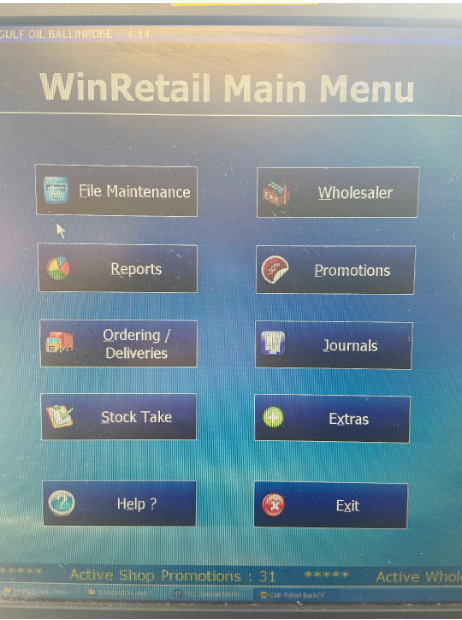
\includegraphics[width=0.25\textwidth]{images/mace1.PNG}
\end{figure}

\begin{figure}[h!]
	\caption{CBE's System in my workplace 2:}
	\label{image:mace2}
	\centering
	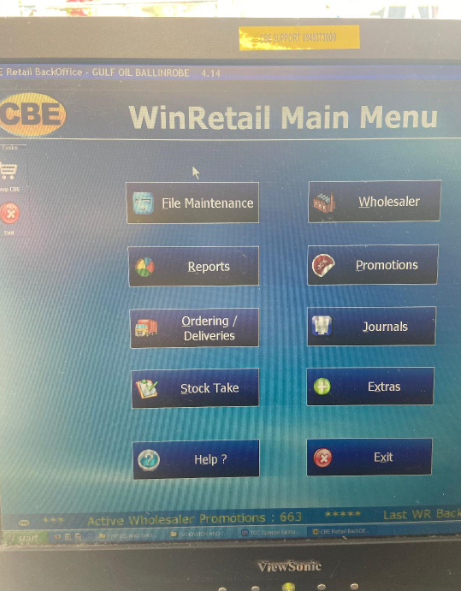
\includegraphics[width=0.25\textwidth]{images/mace2.PNG}
\end{figure}

\begin{figure}[h!]
	\caption{CBE's System in my workplace 3:}
	\label{image:mace3}
	\centering
	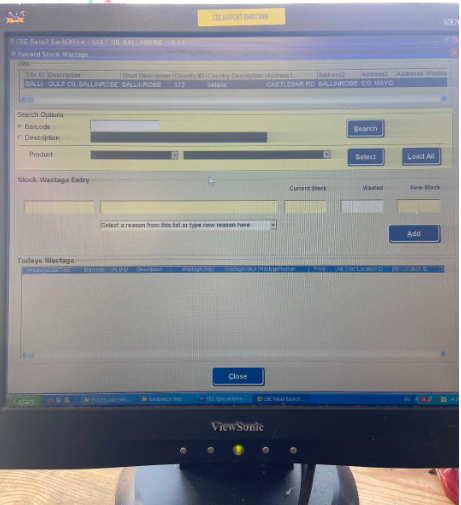
\includegraphics[width=0.25\textwidth]{images/mace3.PNG}
\end{figure}

\begin{figure}[h!]
	\caption{CBE's System in my workplace 4:}
	\label{image:mace4}
	\centering
	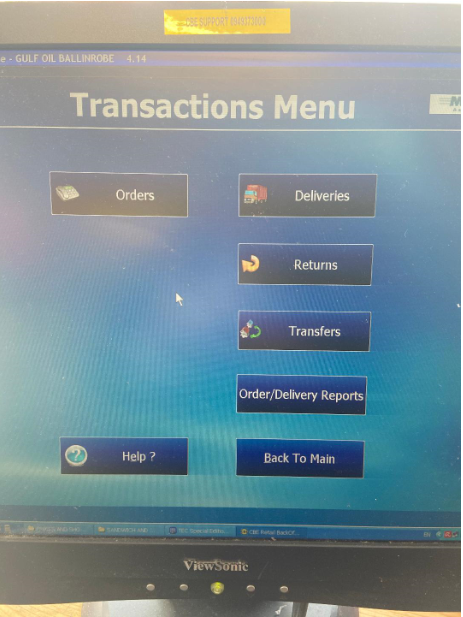
\includegraphics[width=0.25\textwidth]{images/mace4.PNG}
\end{figure}

\begin{figure}[h!]
	\caption{CBE's System in my workplace 5:}
	\label{image:mace5}
	\centering
	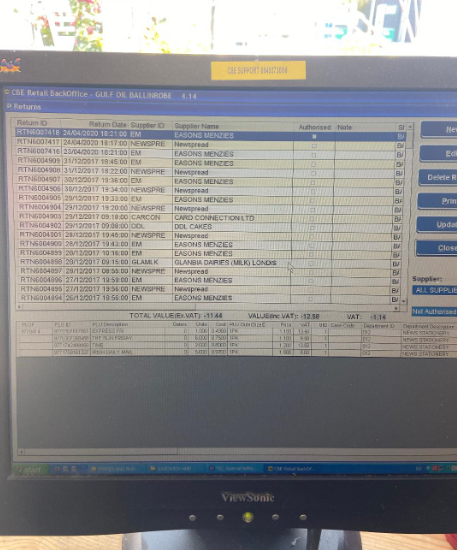
\includegraphics[width=0.25\textwidth]{images/mace5.PNG}
\end{figure}

As you can see in the images above, this is an example taken from the shop i work in. The system provided by CBE that gives reports, wastage, returns details and so on. You can also enter in the delivery dockets here to keep track of your stock but what i am trying to implement is not here. As humans we are expected to find the products that are close or past their sell by date, customers may have a better eye than us and find products that we missed and purchase them deeming them ineffective or dangerous for consumption. My application helps address this existing issue and prevents customer harm and helps the retailers save money and being able to act quickly. To conclude i do believe this application is beneficial and sufficient and based on the survey results my fellow staff members and superiors also think so. 

\subsection{Minor Survey}
In order to prove the idea of implementing a Date Control Application into the workplace is a good idea and will benefit and not hinder staff members, i conducted a short survey, as you can see in the Fig below.

\begin{figure}[h!]
	\caption{Short Survey for Colleagues at work.}
	\label{image:survey}
	\centering
	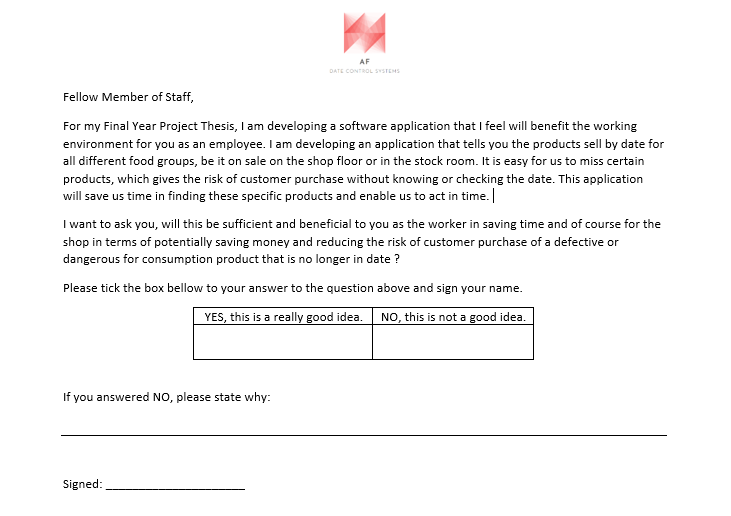
\includegraphics[width=0.8\textwidth]{images/AF-Date-Control-Survey.PNG}
\end{figure}

This is a second opinion that will influence in creating this application. Hearing different opinions being positive or negative is always good. Even if a negative response is given, it will highlight the pros and cons of this application in a more controlled environment. Does that person think it will benefit them, are they a fan of technology, they may prefer physically looking themselves rather than using an application to find things even if it may take longer in which in creating this application i am trying to save my fellow staff members time with the implementation of this application into the workplace, however everyone is entitled to their opinion. 
\newline

This was a major factor in the making and outcome of the application as it gave me more information on what to implement and not implement. I needed to make this application easy to use and understand and to make the application functionality not too complex, making it quick and easy to use for staff and managers. This survey helped in getting a second opinion from someone working in the same role as me. I obviously got opinions from fellow students and my supervisor which were relevant but to get feedback from those who will mainly be using this application was vital in the making of this application and to get an opinion from those who will be using it.
\newline

The results from this survey are in the System Evaluation section of this dissertation. 

\subsection{Planning The Project}
The Planning of this project took place in the first semester for final year where we were told who our project supervisors would be. Once we were told who our supervisors would be i agreed to meet with my supervisor once a week. I am in full support of the provision of supervisors for the Applied Project and Minor Dissertation as it benefited me hugely in the planning of this project. 
\newline

For the first couple of weeks i came to my supervisor with a few different ideas. One of them was this Date Control Application i ended up developing. The other two was to make a more sufficient and more operational version of the group project i contributed to in third year which was an ionic firebase application and a game in C Sharp. The Date Control Application stood out from the offset and the weeks that followed. After many discussions in person and via email i decided to take up this project as my final year project. When this was decided i needed to decide what technology i was going to use and needed to find out has it been done before or similar. 
\newline

After thorough research on the topic i came to the conclusion that this type of application was not done before or if it was it was done by someone as a minor or private application. I discussed the prospect of introducing this idea to CBE once near completion as i felt not only would it benefit retail it would benefit a company that provides shops with their tills and store databases of stock to potentially link my application in some form to their system to save them time and money and even gain customers through this latest potential technology. 
\newline

I also got in touch with my colleagues and superiors at my workplace to get their view on the idea of using an application to help them get stock before it's sell by date and take action and catch everything in the store, be it shop floor stock or back stock where the human eye may not catch. Knowing from experience this is an existing issue, i have missed products in the shop that my colleague might find the next day. I conducted a mini survey within the workplace and put the results in a graph which you will see in the system evaluation section of this write up. 
\newline

The next phase of planning was to decide on what technology i was to use to develop this program. Due to the experience of using Firebase for the first time in third year i made the easy decision to go with Firebase as a database host for my project. Having done Ionic Firebase in third year for the end of year group project there i wanted to give something else a go. So i decided to go with Angular Firebase. Lucky enough for me there is a range of different tutorials on Angular Firebase. I made this decision over the Christmas holidays where i decided on the language choice and started sketching some ideas of how i wanted the application to look and what pages/components i wanted to implement into the project. 
\newline

I wanted to implement some elements to my application that may not be present in a CBE add on application or store application. User Authentication was one element that i implemented for thesis purposes that would maybe not be on a CBE application for various reasons such as time for the staff member to register an account or sign into an account, this applications purpose is to save time for staff not hinder them. Also i wanted to implement a product details form due to the limitation of not having a shops database at my disposal, this is included in this application to indicate the purpose of the application. To show product details and when their best before date is. So in terms of a real life situation, User Authentication and a product form wouldn't need to be required for the purpose of this idea. 
\newline

The plan to use Angular Firebase had to change in the early stages of software development for this project. I decided to switch to Ionic Firebase. There are various similarities between angular and ionic but i felt more comfortable with ionic than i did angular and not to mention i liked the end product of an ionic application rather than angular. Thankfully i changed the plan at the early stage of development.

\subsection{Technologies}
The Technologies i used to develop my idea were as follows:
\newline

\begin{figure}[h!]
	\caption{Developed the code in Visual Studio Code.}
	\label{image:vscode}
	\centering
	
\includegraphics[width=0.4\textwidth]{images/vscode.png}
\end{figure}

- Visual Studio Code - The Editor of my choice for coding the project.
\newline
Whenever we received a project from a lecturer, my initial thought was would i be able to develop this project in Visual Studio Code. Out of all the editors we used throughout the four years of study this stands out as my favourite. It is so easy to use and having using it for past projects and the Ionic Firebase project from third year i had no other editor in mind but Visual Studio Code. I like the file views and the smoothness of the editor when developing a program. To develop this project i would open a command prompt inside my project repository directory and type "code ." and it would open up my project in Visual Studio Code. I could do this with any project. I understand it is the more favoured editor among my peers. 
\newline

\begin{figure}[h!]
	\caption{Programming Language of My choosing for SD.}
	\label{image:ionic}
	\centering
	
\includegraphics[width=0.5\textwidth]{images/ionic.png}
\end{figure}
Ionic - The programming language in which i coded my project. For  the four years of software development course in GMIT i studied various different languages such as Java, C++, C, C Sharp, Python, Ruby and many more. I initially decided to got with using Angular as my programming language for my final year project, however it was giving me various issues and i didn't like the way it was turning out so i decided to code this project using the ionic programming language framework. \cite{cheng2018build} Here is an in depth description of building an Ionic Firebase application that i came across in third year that helped me and my project partner in getting started. 
\newline

Ionic enables you to develop applications using web technologies and languages like HTML, CSS, JavaScript, Angular, and TypeScript. Consider Ionic as a front-end software development kit (SDK) for creating a blend of applications. Ionic provides a collection of components that imitate the native look, feel and functionality of each platform, mainly known for mobile applications but also considered for web applications also, the flexibility of Ionic Framework is why i made the decision to switch and the fact that in my opinion it suits what i in-visioned when sketching the pages i wanted and how they look for the user. Examples of these components include buttons, tabs, menus, lists, cards, modals, and so on. However for colors it is not so broad, but they suited what i was trying to implement. At the end of the day this application was not created to look pretty it was created to solve a problem in the work place, a Date Control Problem.
\newline

Out of the four years of studying software development, Ionic and Angular stood out. In my second year of study in GMIT i encountered the Angular Framework, and in third year i encountered the Ionic Framework. When coming up with the idea of creating my Date Control application i wanted to use a language i liked and enjoyed doing. In third year for the group project myself and another student created a cinema booking website using Ionic Firebase. From then i knew i wanted to use Firebase for its easy implementation into the Ionic Framework for an application. As i always want to learn something new, although similar Ionic and Angular are different, as mentioned above i initially started the project in Angular and then switched to Ionic. I did this as i did not feel as comfortable with Angular Firebase as i did with Ionic Firebase. I'm glad i made the switch for a number of reasons including software development, overall design and it's link to the Firebase DB Cloud.
\newline

\begin{figure}[h!]
	\caption{Cloud Database of My choosing for Data Storage.}
	\label{image:fire-base}
	\centering
	
\includegraphics[width=0.5\textwidth]{images/fire-base.png}
\end{figure}

- Firebase - The Cloud Database i used to store User Authentication details and store the product entry data for crud functionality. Note for private and security purposes i the admin of the Firebase database cannot see what the users passwords are, firebase hash them in which i or anyone else does not know. Within visual studio code in my software development to connect my firebase database project made on firebase i had to implement unique firebase configuration values to my environments files. It should look something like this if you were to ever take up a project with firebase.   
\newline

\begin{figure}[h!]
	\caption{Example of Firebase Configuration:}
	\label{image:firebaseConfig}
	\centering
	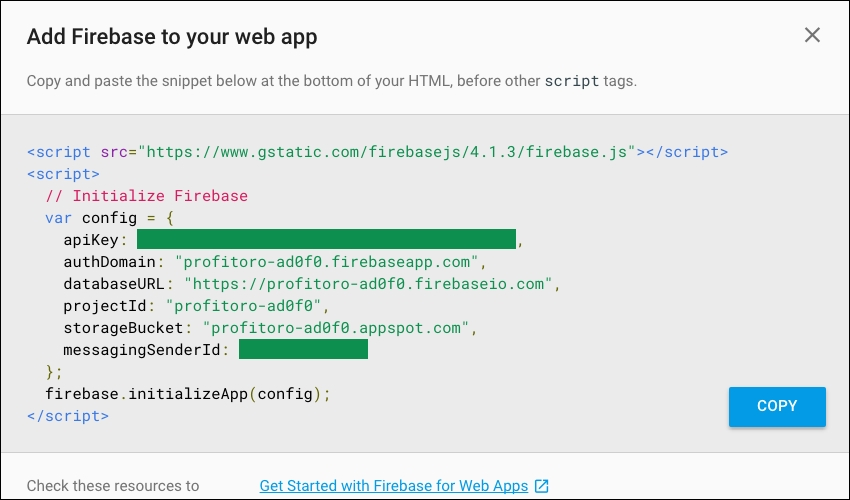
\includegraphics[width=0.5\textwidth]{images/firebaseConfig.jpg}
\end{figure}

\begin{figure}[h!]
	\caption{All Project Items are on GitHub and can be cloned.}
	\label{image:github1}
	\centering
	
\includegraphics[width=0.4\textwidth]{images/github.png}
\end{figure}

- GitHub - I used to publish my project on the internet for the thesis and for people to then test themselves. GitHub gives a brief description of the project as a whole and explains to the person wishing to test how to run or try out the application. 
\newline

\begin{figure}[h!]
	\caption{This project dissertation was edited on Overleaf in LaTeX.}
	\label{image:overleaf-latex}
	\centering
	
\includegraphics[width=0.4\textwidth]{images/overleaf-latex.png}
\end{figure}
\newpage
- Overleaf - I used overleaf as a Latex editor for this project dissertation. I used this template provided to us from our year head. I only came across Overleaf with LaTeX in the first semester of final year where much like this section we needed to create a Literature review. This benefited me in terms of writing this dissertation.

\subsection{Issues}

\begin{figure}[h!]
	\caption{In Every Project or Idea Issues arise.}
	\label{image:issues}
	\centering
	
\includegraphics[width=0.4\textwidth]{images/issues.jpg}
\end{figure}

In every project or idea issues can very easily arise. During the software development you may encounter issues such as compile errors, server errors, and maybe some code implemented that worked on older versions of software, for example, some functions or declarations that work on Ionic 2 wont work on Ionic 5 and so on. HTML issues such as buttons not working, pages not showing due to an error in the code and so on. Issues can very easily arise in any software projects, in fact make that any project whatsoever. In this section i will be discussing the issues that arose for me during the software development part of the project. 
\newline

The first issue arose when i decided to pursue the Date Control Application in Angular Firebase. Having done Ionic Firebase in Third Year for the group project i wanted to challenge myself in trying out Angular with Firebase. Having set up the authentication with Angular Firebase i didn't like the way it was looking and what it was going to look like when implementing the CRUD functionality to the application. I feel here in the end it was the correct decision in the long run. I referenced my third year project a lot during the making of this application as it too was Ionic Firebase. In terms of experience this worked in my favour. 
\newline

I then realised that i wanted to pursue this project in Ionic. I made the switch which you can see in the early commits of the software development of the project. I made the switch of course for the reasons mentioned, however i also switched due to the fact i was familiar with Ionic Firebase having completing a project in it before. I liked the look overall of Ionic. This did not hinder me to much in the completion of this application. At that stage i was at the stage of testing the waters, what will and won't work and how it will look in the end. This wasn't a major issue and i was glad i made the switch. 
\newline

The Next issue that arose was the authentication "reset/forgot" password. After looking at many different tutorials online i was unable to get this function to work. The code is still in the project directory but has to be commented out due to ionic build errors when trying to make the project a Firebase hosted website. Due to the fact if CBE were to implement this application into their systems they may not have the idea of a user authentication system within it, as this is a prototype i feel it does not hinder the overall reasoning for this application. A password reset email can be sent via the Firebase console to the user upon request. This issue is highlighted in the issues section of the GitHub Repository for this project.
\newline

Another issue that stood out was the sorting issue. I wanted to sort the data read into the Firebase Cloud Database to be loaded into the food groups pages with the best before date closest to the current date to be at the top of the list. Unfortunately this feature was not implemented. I tried various different ways to implement it such as a query in the get product details function and also the fetch product details functionality that shows the product details on the page. I even tried to alter the Firebase database to show this by trying to implement rules to do so. I was unable to make this feature work, however the idea was there and may be implemented if taken up by the likes of CBE who may take a different approach in showing data in this format. This issue is highlighted in the issues section of the GitHub Repository for this project.
\newline

A Small bug started to arise when signing into an account also. Where a window pop up gives an error message along the lines of "null is not an object". This issue is also highlighted on GitHub. This does not hinder a sign in, as if you click the log in button again it will sign you in.
\newline

Thankfully no major issues arose that i expected to arise, for example when making this application a Firebase hosted website i had the fear of when trying to do this will result in the application breaking completely. Since this was at a late stage it was a very fragile time in the software development phase. 

\newpage
\subsection{Technology References}
\url{https://developer.okta.com}
\newline
\url{https://ionicframework.com/docs/theming/colors}
\newline
\url{https://ionicframework.com/docs/building/running}
\newline
\url{https://www.tutorialspoint.com/ionic/ionic_colors.htm}
\newline
\url{https://ionicons.com/}
\newline
\url{https://www.youtube.com/watch?v=M-nTpVIyGw0}
\newline
\url{https://devdactic.com/host-ionic-website-firebase/}
\newline
\url{https://forum.ionicframework.com/t/how-to-add-styles-to-ion-button-inner-text/148987}
\newline
\url{https://ionicframework.com/docs/native/firebase-authentication}
\newline
\url{https://www.freakyjolly.com/ionic-firebase-crud-operations/#.XrKlWqhKjIU}
\newline
\url{https://github.com/AndreasFahey/ajproject}

